\chapter{Markdown for Git plugin}

This milestone covers the development of the \ref{gloss:markdown} for \ref{gloss:git} plugin described in stage \ref{num:stage10} of the \Nameref{sec:developmentStages}.

\section{Plugin structure}

The \ref{gloss:markdown} for \ref{gloss:git} plugin will be composed of components developed in \Nameref{chap:processingLibraries}.

\begin{figure}[H]
    \centering
    \label{fig:pluginStructure}
    \tikzset{every picture/.style={line width=0.75pt}} %set default line width to 0.75pt

        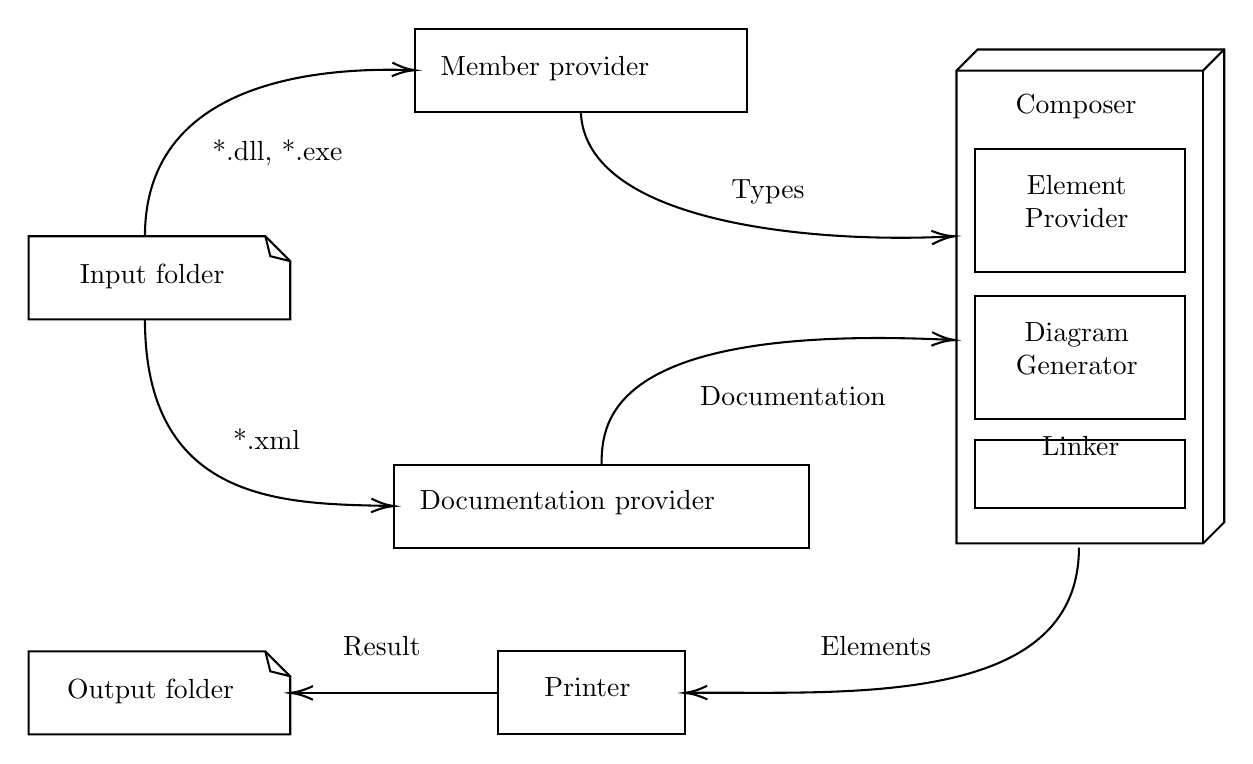
\begin{tikzpicture}[x=0.75pt,y=0.75pt,yscale=-1,xscale=1]
        %uncomment if require: \path (0,428); %set diagram left start at 0, and has height of 428

        %Shape: Folded Corner [id:dp38453805550218356]
        \draw   (128,110) -- (14,110) -- (14,150) -- (140,150) -- (140,122) -- cycle -- (128,110) ; \draw   (140,122) -- (130.4,119.6) -- (128,110) ;

        %Shape: Cube [id:dp9514351083967096]
        \draw   (461,30.21) -- (471.21,20) -- (590,20) -- (590,247.79) -- (579.79,258) -- (461,258) -- cycle ; \draw   (590,20) -- (579.79,30.21) -- (461,30.21) ; \draw   (579.79,30.21) -- (579.79,258) ;
        %Shape: Rectangle [id:dp28951515389797833]
        \draw   (470,68) -- (571,68) -- (571,127) -- (470,127) -- cycle ;

        %Shape: Rectangle [id:dp811482931901953]
        \draw   (470,208) -- (571,208) -- (571,241) -- (470,241) -- cycle ;

        %Shape: Rectangle [id:dp5590157968822316]
        \draw   (470,139) -- (571,139) -- (571,198) -- (470,198) -- cycle ;


        %Shape: Rectangle [id:dp0837615901192712]
        \draw   (200,10) -- (360,10) -- (360,50) -- (200,50) -- cycle ;

        %Shape: Rectangle [id:dp21181013544630467]
        \draw   (190,220) -- (390,220) -- (390,260) -- (190,260) -- cycle ;

        %Curve Lines [id:da5699658849973097]
        \draw    (70,110) .. controls (70,31.86) and (161.2,28.74) .. (198.34,29.94) ;
        \draw [shift={(200,30)}, rotate = 182.12] [color={rgb, 255:red, 0; green, 0; blue, 0 }  ][line width=0.75]    (10.93,-3.29) .. controls (6.95,-1.4) and (3.31,-0.3) .. (0,0) .. controls (3.31,0.3) and (6.95,1.4) .. (10.93,3.29)   ;
        %Curve Lines [id:da0934002278421866]
        \draw    (70,150) .. controls (70,240.75) and (140.57,238.72) .. (188.55,239.96) ;
        \draw [shift={(190,240)}, rotate = 181.59] [color={rgb, 255:red, 0; green, 0; blue, 0 }  ][line width=0.75]    (10.93,-3.29) .. controls (6.95,-1.4) and (3.31,-0.3) .. (0,0) .. controls (3.31,0.3) and (6.95,1.4) .. (10.93,3.29)   ;
        %Curve Lines [id:da9139301607505403]
        \draw    (280,50) .. controls (281.98,104.12) and (393.73,113.48) .. (458.07,110.11) ;
        \draw [shift={(460,110)}, rotate = 176.72] [color={rgb, 255:red, 0; green, 0; blue, 0 }  ][line width=0.75]    (10.93,-3.29) .. controls (6.95,-1.4) and (3.31,-0.3) .. (0,0) .. controls (3.31,0.3) and (6.95,1.4) .. (10.93,3.29)   ;
        %Curve Lines [id:da360087403261089]
        \draw    (290,220) .. controls (290,198.67) and (294,151.67) .. (460,160) ;
        \draw [shift={(460,160)}, rotate = 182.87] [color={rgb, 255:red, 0; green, 0; blue, 0 }  ][line width=0.75]    (10.93,-3.29) .. controls (6.95,-1.4) and (3.31,-0.3) .. (0,0) .. controls (3.31,0.3) and (6.95,1.4) .. (10.93,3.29)   ;
        %Shape: Rectangle [id:dp5335135464926624]
        \draw   (240,310) -- (330,310) -- (330,350) -- (240,350) -- cycle ;

        %Curve Lines [id:da34448081447371903]
        \draw    (520,260) .. controls (520,338.61) and (403.18,329.1) .. (331.08,329.99) ;
        \draw [shift={(330,330)}, rotate = 359.2] [color={rgb, 255:red, 0; green, 0; blue, 0 }  ][line width=0.75]    (10.93,-3.29) .. controls (6.95,-1.4) and (3.31,-0.3) .. (0,0) .. controls (3.31,0.3) and (6.95,1.4) .. (10.93,3.29)   ;
        %Shape: Folded Corner [id:dp9495985347442353]
        \draw   (128,310) -- (14,310) -- (14,350) -- (140,350) -- (140,322) -- cycle -- (128,310) ; \draw   (140,322) -- (130.4,319.6) -- (128,310) ;
        %Straight Lines [id:da8650986253114432]
        \draw    (240,330) -- (142,330) ;
        \draw [shift={(140,330)}, rotate = 360] [color={rgb, 255:red, 0; green, 0; blue, 0 }  ][line width=0.75]    (10.93,-3.29) .. controls (6.95,-1.4) and (3.31,-0.3) .. (0,0) .. controls (3.31,0.3) and (6.95,1.4) .. (10.93,3.29)   ;

        % Text Node
        \draw (37.11,122) node [anchor=north west][inner sep=0.75pt]   [align=left] {Input folder};
        % Text Node
        \draw (485,79) node [anchor=north west][inner sep=0.75pt]   [align=left] {\begin{minipage}[lt]{48.65pt}\setlength\topsep{0pt}
        \begin{center}
        Element\\Provider
        \end{center}

        \end{minipage}};
        % Text Node
        \draw (499,205) node [anchor=north west][inner sep=0.75pt]   [align=left] {\begin{minipage}[lt]{30.51pt}\setlength\topsep{0pt}
        \begin{center}
        Linker
        \end{center}

        \end{minipage}};
        % Text Node
        \draw (485,150) node [anchor=north west][inner sep=0.75pt]   [align=left] {\begin{minipage}[lt]{48.65pt}\setlength\topsep{0pt}
        \begin{center}
        Diagram\\Generator
        \end{center}

        \end{minipage}};
        % Text Node
        \draw (488,40) node [anchor=north west][inner sep=0.75pt]   [align=left] {Composer};
        % Text Node
        \draw (211,22) node [anchor=north west][inner sep=0.75pt]   [align=left] {Member provider};
        % Text Node
        \draw (201,231) node [anchor=north west][inner sep=0.75pt]   [align=left] {Documentation provider};
        % Text Node
        \draw (101,62) node [anchor=north west][inner sep=0.75pt]   [align=left] {*.dll, *.exe};
        % Text Node
        \draw (111,201) node [anchor=north west][inner sep=0.75pt]   [align=left] {*.xml};
        % Text Node
        \draw (351,81) node [anchor=north west][inner sep=0.75pt]   [align=left] {Types};
        % Text Node
        \draw (336,181) node [anchor=north west][inner sep=0.75pt]   [align=left] {Documentation};
        % Text Node
        \draw (261,321) node [anchor=north west][inner sep=0.75pt]   [align=left] {Printer};
        % Text Node
        \draw (394,301) node [anchor=north west][inner sep=0.75pt]   [align=left] {Elements};
        % Text Node
        \draw (31,322) node [anchor=north west][inner sep=0.75pt]   [align=left] {Output folder};
        % Text Node
        \draw (164,301) node [anchor=north west][inner sep=0.75pt]   [align=left] {Result};
    \end{tikzpicture}
    \caption{Plugin components structure}
\end{figure}

Figure \ref{fig:pluginStructure} depicts relations between each component, the input folder, and the output folder. The member and documentation providers operate in parallel, and supply necessary data to the composer component by processing files from the input folder.
The composer component depends on the element provider, linker, and diagram generator for composing the extracted data into a structured documentation.
Finally, the structured documentation is fed into the printer component, which simply generated the physical files into the designated output folder.

\section{Plugin configuration steps}

The plugin must provide configuration steps for the user to set how each component should operate. It is not necessary for the plugin to provide configuration steps for every component, as some might not be configurable. Additionally, the plugin might provide configurations that affect more than one component.

In the case of the \ref{gloss:markdown} for \ref{gloss:git} plugin, the following configuration steps are necessary in this order specifically:
\begin{itemize}
    \item Member provider
    \item Documentation provider
    \item Linker
    \item Global configuration
\end{itemize}

\subsection{Member provider}

The member provider configuration would be labeled to the user as the \textbf{Assembly} processing component, because the they would select the desired assemblies and executable \ref{gloss:dotnetlabel} files for processing.

The user can move to the next step once at least one file is provided.

\subsubsection{Mock}

\begin{figure}[H]
    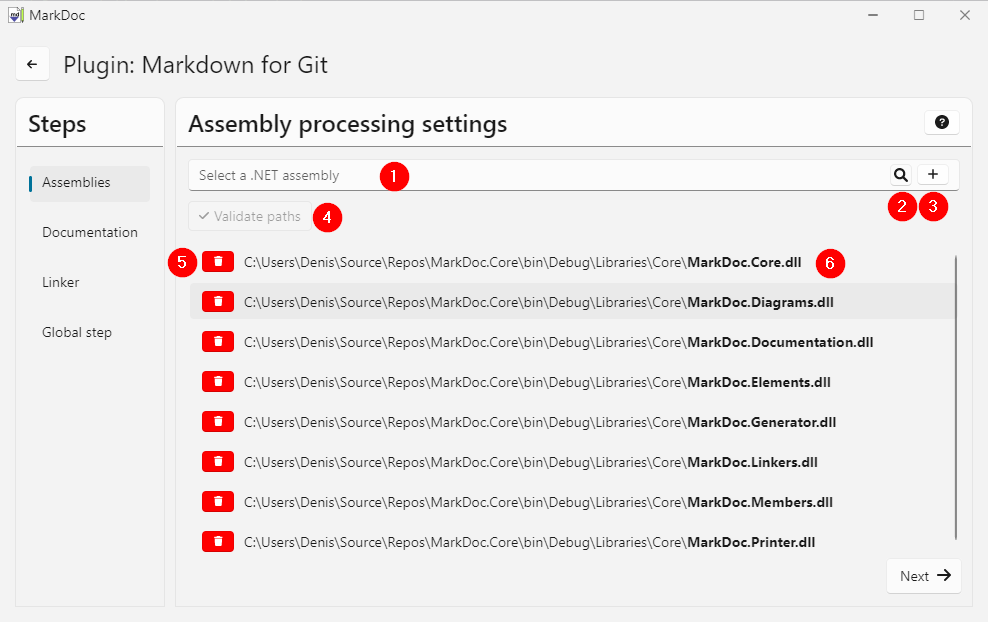
\includegraphics[width=\linewidth]{img/pluginMember.png}
    \label{fig:pluginMember}
    \caption{Assembly configuration step}
\end{figure}

\begin{enumerate}
    \item Text field for manually entering the assembly or executable for processing
    \item Button for browsing the system for the desired assemblies of executables for processing
    \item Button for adding the manually entered path
    \item Button for revalidating the provided file paths for their existence and system permissions (not implemented, disabled)
    \item Button for removing the added file path
    \item The added file path with the file highlighted in bold
\end{enumerate}

\subsection{Documentation provider}

The documentation provider step displays the automatically discovered documentation files, alongside those that are missing. Unfortunately, this configuration step does not allow ignoring, or manually specifying documentation file paths, because of limited development time.

\subsubsection{Mock}

\begin{figure}[H]
    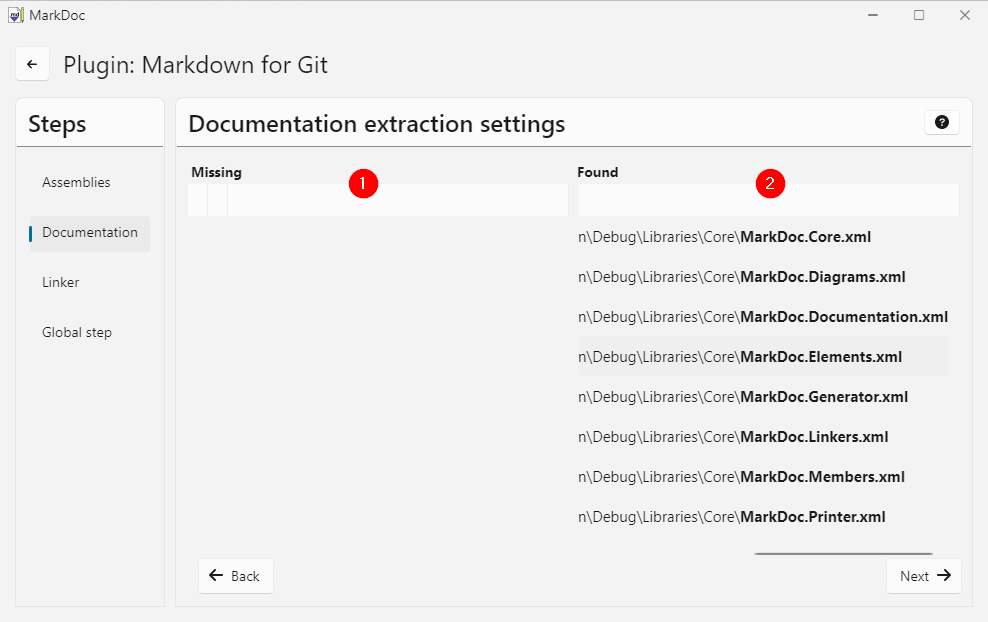
\includegraphics[width=\linewidth]{img/pluginDocumentation.png}
    \label{fig:pluginDocumentation}
    \caption{Documentation configuration step}
\end{figure}

\begin{enumerate}
    \item Table with a list of missing documentation files
    \item Table with a list of located documentation files
\end{enumerate}

\subsection{Linker}

The linker step displays configuration options that target specific \ref{gloss:git} platforms. The user can generate documentation either for GitHub or GitLab. The choice affects the generated link format, which is platform-specific.

Next, they can decide whether the documentation will be hosted in the repository alongside the source code, or the Wiki pages. This option is necessary for GitHub, since its Wiki limits its users to a flat file structure, whereas GitLab allows structuring documentation into folder in their Wiki. Moreover, GitHub does not allow uploading multiple pages to the Wiki in bulk. Thus, if there is a lot of documentation, a user would most likely need to use the option for hosting documentation alongside the source code.

Finally, it is possible to explicitly choose whether the documentation is generated flat, or structured into individual folders. This option is relevant for GitLab, as it allows both.

\subsubsection{Mock}

\begin{figure}[H]
    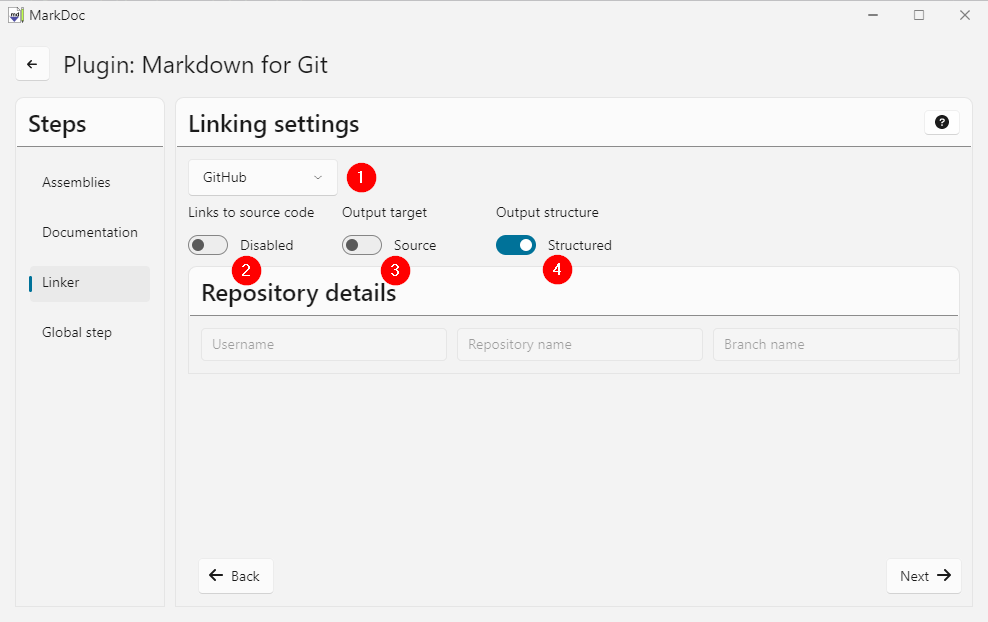
\includegraphics[width=\linewidth]{img/pluginLinker.png}
    \label{fig:pluginLinker}
    \caption{Linker configuration step}
\end{figure}

\begin{enumerate}
    \item Selection of the target \ref{gloss:git} system
    \item Toggle for linking generated documentation to source files (not implemented, disabled)
    \item Toggle for determining whether the generated output will be stored with the source code, or the Wiki
    \item Toggle for determining whether the generated output will be structured into multiple subfolders, or flat
\end{enumerate}

\subsection{Global configuration}

The global configuration affects all components, as it provides a filter for excluding specific namespaces and types from being processed. Additionally, it allows users to specify the output folder for the generated documentation.

\subsubsection{Mock}

\begin{figure}[H]
    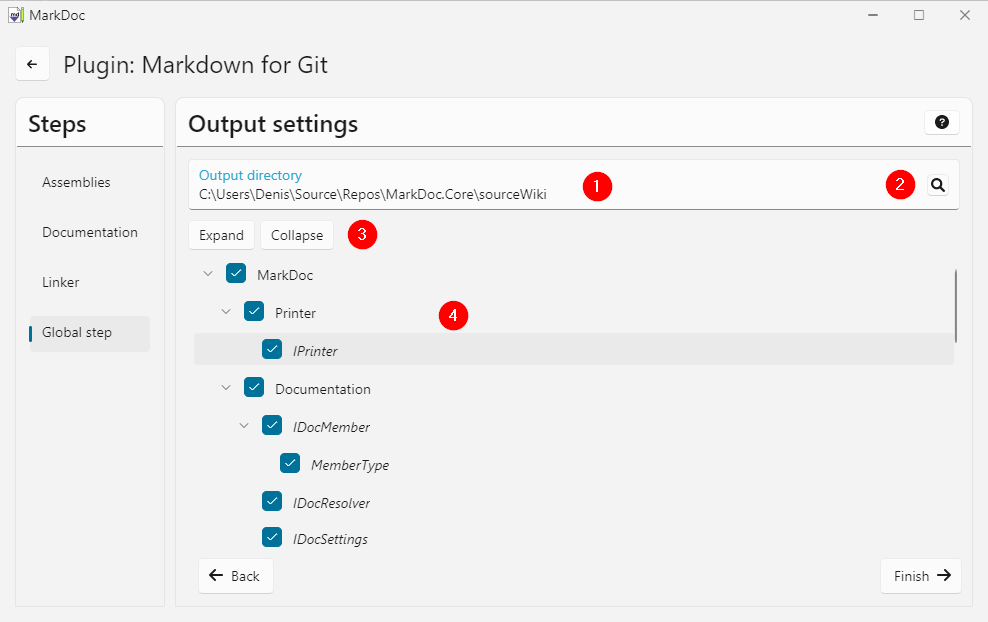
\includegraphics[width=\linewidth]{img/pluginGlobal.png}
    \label{fig:pluginGlobal}
    \caption{Global configuration step}
\end{figure}

\begin{enumerate}
    \item Output path for the generated documentation
    \item Button for browsing the output path
    \item Buttons for toggling the expansion and collapsing of the namespace and type tree
    \item The namespace and type tree for toggling what entries are to be removed from the processing
\end{enumerate}